\chapter{2D Janssen effect in a friction-driven system}
\author{Mohammad Yasinul Karim, Eric I. Corwin}


This chapter includes work that has been published in Physical Review Letters volume 112 on May 9, 2014. The experimental design, data collection and analysis was done by me with guidance from my advisor, Eric Corwin, who is a co-author on the paper. 

\section{Background}

The Janssen effect is a unique property of confined granular materials experiencing gravitational compaction in which the pressure at the bottom saturates with increasing filling height due to frictional interactions with side walls. In this paper we replace gravitational compaction with frictional compaction.  We study friction-compacted 2D granular materials confined within fixed boundaries on a horizontal conveyor belt. We find that even with high friction side walls the Janssen effect completely vanishes. Our results demonstrate that gravity-compacted granular systems are inherently different from friction-compacted systems in at least one important way: vibrations induced by sliding friction with the driving surface relax away tangential forces on the walls. Remarkably, we find that the Janssen effect can be recovered by replacing the straight side walls with a sawtooth pattern. The mechanical force introduced by varying the sawtooth angle $\theta$ can be viewed as equivalent to a tunable friction force. By construction, this mechanical friction force cannot be relaxed away by vibrations in the system.

This work was originally published in \textit{Physical Review Letters}.  The writing and analysis were performed by me as primary author.  Eric Corwin is listed as a coauthor as he advised this work.  

Granular materials in bulk can exhibit liquid-like, solid-like or gas-like behavior \cite{jaeger_physics_1992, jaeger_granular_1996, liu_nonlinear_1998, trappe_jamming_2001}. There are few illustrations of this more striking than the Janssen  effect in a grain-filled silo.  The Janssen effect describes the saturation of bottom pressure with increasing filling height in a static 3D system of granular particles confined in a container with vertical walls \cite{janssen_versuche_1895, duran_sands_2000, sperl_experiments_2006}. If an empty silo is gradually filled with a frictional granular material a measurement at the bottom will initially show pressure increasing linearly with filling height. However, as the filling height becomes equal to the width of the silo the measured pressure at the bottom begins to saturate, asymptoting to a constant value independent of filling height. As the granular material is compressed by the weight of the material above, it presses down on the material below and outwards on the confining walls. This creates a large normal force against the walls which allows for the mobilization of a large frictional tangential force between individual grains and the confining walls. Thus, in a tall silo the majority of the vertical force is actually borne by the walls of the silo. This is in striking contrast to a silo filled with liquid, in which the walls will only experience normal forces and thus carry none of the vertical load. 
%
\begin{figure}
	\includegraphics[width=\textwidth]{Figures/chapter2/conveyor}
	\caption{Diagram of the experimental setup. The nickels are driven by the belt into a 2D container that is stationary. The nickels are blocked at one end by an acrylic barrier which presses against two force sensors A and B as the nickels accumulate against this surface. The nickels are confined on the sides by walls constructed from ABS and with sawtooth patterns engraved on the sides facing the nickels. The arrow points towards direction of conveyor belt.}
	\label{fig:conveyor}
\end{figure}
%

Vertical, gravity compacted 3D granular packings and granular hopper flows have been well studied \cite{nedderman_flow_1982, kadanoff_built_1999, de_gennes_granular_1999,  bertho_dynamical_2003, landry_confined_2003, mankoc_flow_2007, hilton_granular_2011}. However, industrial processes as diverse as coal mining, grain storage, oil extraction, and pharmaceutical manufacture, to name only a few, rely on granular materials being transported horizontally on conveyor belts. In recent works Aguirre, \textit{et al.} have examined hopper flows in 2D granular systems where grains are loaded horizontally by a conveyor belt into a confining frame. They measured the flow rates of grains escaping through an aperture for varying aperture sizes and belt speeds \cite{aguirre_pressure_2010} and also the normal forces on the base during the granular discharge \cite{aguirre_granular_2011}. The results show that for a given aperture size, the hopper flow rate remains constant even though the pressure at the base changes as the grains leave the frame. They conclude that the Janssen effect, which in previous studies was invoked to explain the constant hopper flow rates, is irrelevant.  Instead, the study shows that it is the local pressure near the aperture that determines the flow rate. However, they did not explore static packings and their experiments were limited to relatively short packings (ratio of maximum filling height to system width $\approx$ 2).

In this paper we present a direct investigation of the Janssen effect in confined 2D granular systems with no flow, compacted by dynamic friction.  We find that in a 2D horizontal container with straight confining walls the pressure at the bottom increases linearly with filling height, demonstrating that the effective particle-wall friction is reduced to zero. Sawtooth walls have been used in 2D \cite{farkas_segregation_2002, mobarakabadi_granular_2013} and 3D \cite{derenyi_collective_1998, farkas_transitions_1999} granular systems to tune the dynamic motion of grains in an excited system.  Here we use them to change the boundary conditions of a static system. In this experiment we show that a sawtooth pattern can be employed in a static, friction-compacted granular system to recover a Janssen-like behavior. 

We can write the expected Janssen equation for a 2D friction driven system by replacing the force of gravity with a downstream pointing dynamic friction force on each particle of $\mu_{pb} m g$, where $\mu_{pb}$ is the coefficient of dynamic friction between a particle and the belt, $m$ is the mass of a particle, and $g$ is acceleration due to gravity. The 2D pressure $F/w$, where $F$ is the total force at the bottom of the system and $w$ is the effective width of the container, can be written as a function of the filling height $x$ as
%
\begin{equation} 
\frac{F}{w}=\mu_{pb} \rho g \eta (1 - \exp(-x/\eta))
\label{eq:janssen}
\end{equation}
%
where $\eta$ is the characteristic height for saturation of pressure and $\rho$ is the 2D density.

In Janssen's calculation the normalized characteristic height $\eta/w$ is
\begin{equation} 
\frac{\eta}{w}=\frac{1}{2K\mu_{pw}}
\label{eq:eta}
\end{equation}
where $K$ is the ratio of horizontal pressure to vertical (downstream) pressure at any point in the granular system and $\mu_{pw}$ is the particle-wall coefficient of friction. As in the gravity driven case, we make the simplifying assumption that $K$ is constant throughout the entire system \cite{janssen_versuche_1895, sperl_experiments_2006, duran_sands_2000}.


%\section{Experiments}

Figure \ref{fig:conveyor} shows our experimental setup which consists of nickels in a horizontal 2D container on top of a $10$ foot variable speed conveyor (McMaster-Carr 5900K786 with a Forbo Siegling PVC belt.  We choose nickels as our granular particles due to their precise manufacture, large coefficient of friction, and their ability to resist buckling under compression.  We measure the 2D bulk density of jammed nickels to be $\simeq$ 11.45 kg/m$^{2}$. The coefficient of dynamic friction between particles and the belt is measured to be $\mu_{pb} \simeq 1$.  Our container consists of fixed sidewalls and a freely moving downstream barrier.  The ends of the downstream barrier are mounted on rails so that the total force at the bottom of the packing can be measured by the two force sensors (Measurement Specialties FC22) and recorded digitally (National Instruments NI USB-6009).  The sidewalls and the downstream barrier are held $\simeq$0.25 mm above the conveyor belt to prevent escape of the 1.95 mm tall nickels while avoiding contact between the belt and the walls.  The sidewalls are 3D printed in ABS plastic for a range of sawtooth angles $\theta$ using a Makerbot Replicator 2X. The repeat spacing of the sawtooth patterns is chosen to be 25.4 mm, slightly larger than the diameter of a nickel (21.21 mm).  For each $\theta$ we adjust the spacing of the sidewalls to maintain a constant increase in average filling height of 7.6 cm for every 30 nickels added. The effective width $w$ of the system is calculated as a fit parameter from Equation \ref{eq:janssen} at each $\theta$ and these values are plotted in Figure \ref{fig:collapse} inset. 


For each $\theta$ we measure the force at the downstream barrier as a function of filling height.  We make each measurement by randomly distributing thirty nickels upstream on the conveyor belt and allowing them to come to rest within the container.  After they have been deposited we record the average force $F$ over a span of 30 s and directly measure the filling height $x$.  We continue adding 30 nickels at a time and measuring the force until we reach a maximum filling height of 1.2 m or the nickels buckle.   All measurements are taken with the belt moving at a constant a speed of 14 cm/s. This speed is slow enough that collisions don't result in buckling while still being fast enough for rapid data collection.  

%Figure \ref{fig:pressurevh} shows the results of these measurements for values of $\theta$ ranging from 0-90$^{\circ}$ and clearly demonstrates that as $\theta$ increases the saturation height decreases.

% 
\begin{figure}
	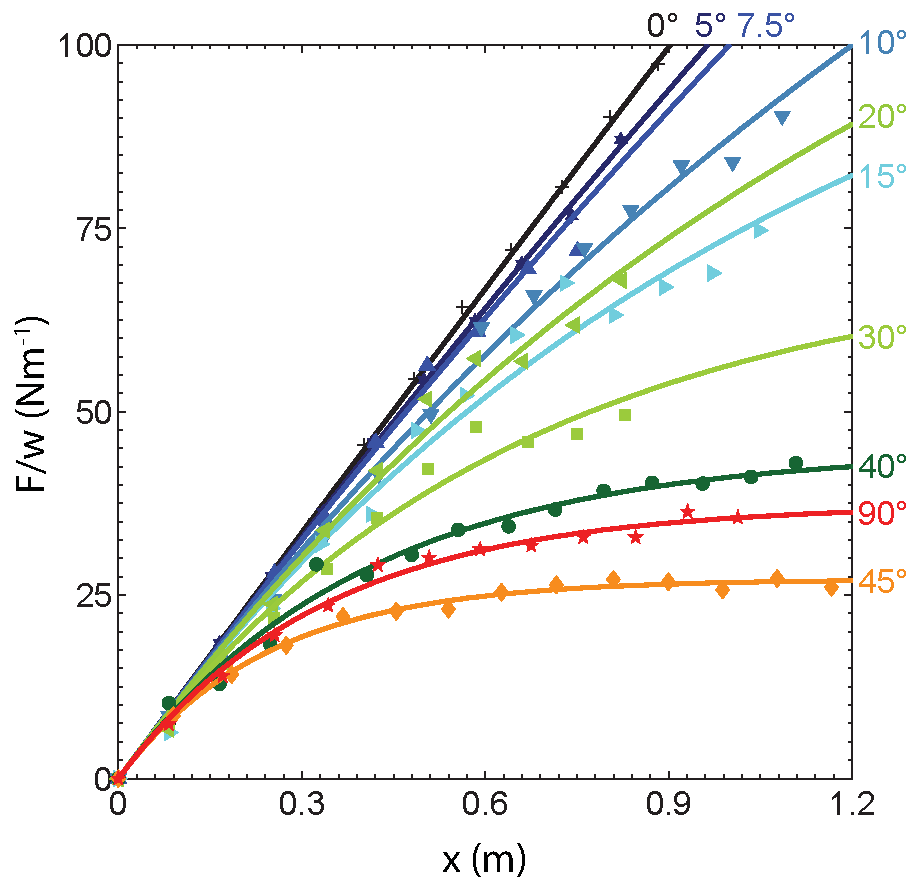
\includegraphics[width=\textwidth]{Figures/chapter2/pressurevh}
	\caption{Measured force $(F)$ per container width $(w)$ is plotted at various filling heights for $\theta = 0^{\circ}$, $5^{\circ}$, $7.5^{\circ}$, $10^{\circ}$, $15^{\circ}$, $20^{\circ}$, $30^{\circ}$, $40^{\circ}$, $45^{\circ}$ and $90^{\circ}$. The data is fitted to the equation $F/w = \mu \rho g \eta (1 - exp(-x/\eta))$ (solid lines). The bottom pressure $(F/w)$ saturates faster with increasing angle of inclination of the triangles along the side walls. At very low angles of inclination ($\theta$ $=$ $0^{\circ}$, $5^{\circ}$, $7.5^{\circ}$) the bottom pressure increases nearly linearly for the observed filling heights.}
	\label{fig:pressurevh}
\end{figure}
%

\section{Results and Discussion}

Figure \ref{fig:pressurevh} presents experimental data along with 2-parameter fits to Equation \ref{eq:janssen}.  The fits yield values for characteristic height $\eta$ and width $w$.  We use the value of $w$ to plot 2D pressure $F/w$ as a function of filling height $x$.  We find that for $\theta = 0^{\circ}$ (straight walls) the $2D$ pressure $F/w$ increases linearly with filling height, consistent with $\eta = \infty$ and thus $\mu_{pw} = 0$ (Figure \ref{fig:pressurevh}). This is in striking contrast to the predicted scale of $\eta$, which would be of the order $w$ for $\mu_{pw}$ and $K$ of the order 1. Thus, with straight walls, the high-friction granular system consisting of nickels seemingly behaves like a frictionless fluid. In the gravity-driven case, particle-wall friction is fully mobilized unless an outside force is introduced to the system. However, in our conveyor belt driven system, the constant sliding friction of the belt perturbs the nickels so that the particle-wall friction cannot be mobilized. Hence, we see the force of the granular system is completely borne by the base. 

If we replace the straight walls with a sawtooth pattern, however, we recover Janssen-like behavior: $F/w$ initially increases linearly with filling height and then bends over to a plateau for higher filling heights (Figure \ref{fig:pressurevh}).  The plateau value of the 2D pressure decreases with increasing $\theta$, even though the same perturbative sliding friction exists in the system.  We demonstrate that our modified Janssen equation (Equation \ref{eq:janssen}) accurately models the physics of the system by plotting a scaled pressure, $F/(w\mu g\rho\eta)$ versus a scaled filling height, $x/\eta$, as shown in Figure \ref{fig:collapse}.
%
\begin{figure}
	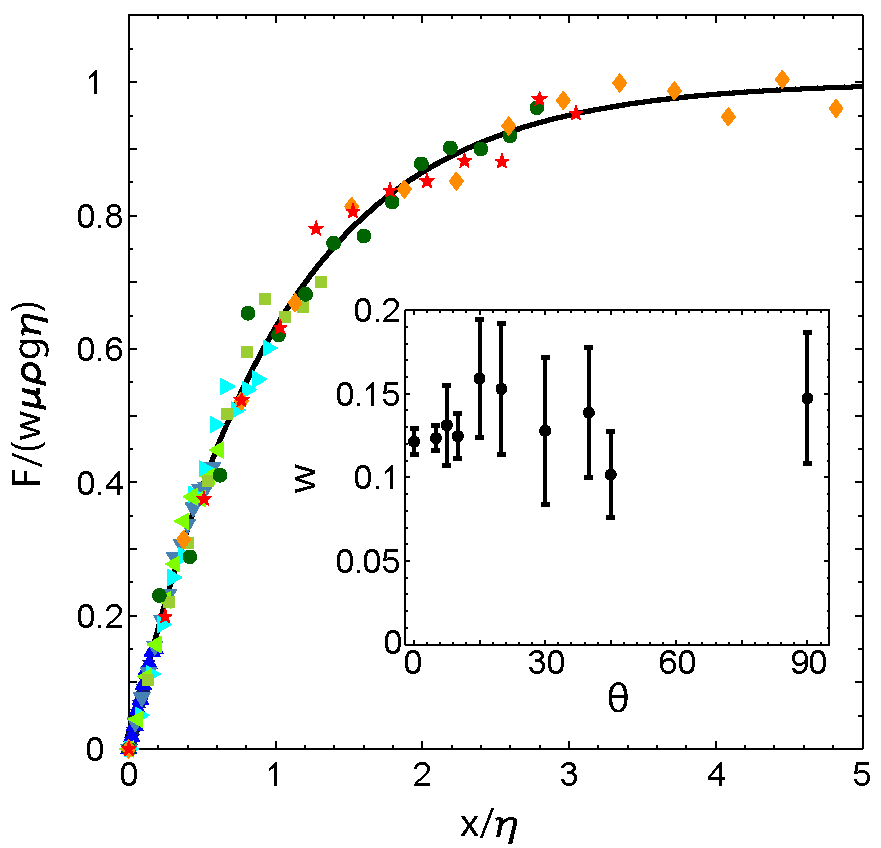
\includegraphics[width=\textwidth]{Figures/chapter2/collapse}
	\caption{The dimensionless quantity $F/(wg\rho\eta)$ is plotted against $x/\eta$ for several values of $\theta$ and all data collapses onto a single master curve given by $ F/(wg\rho\eta) = 1 - exp(-x/\eta)$. Inset is a plot of fitted values of width versus angle of inclination $\theta$.}
	\label{fig:collapse}
\end{figure}
%

Figure \ref{fig:collapse} demonstrates that the sidewalls are bearing much of the downstream force of the system, even in the absence of friction between the particles and the wall.  Instead, this force must have a geometric origin.  To account for this we can modify Equation \ref{eq:eta} to relate the characteristic height to the geometrically determined downstream force on the sidewalls.

%
\begin{figure}
	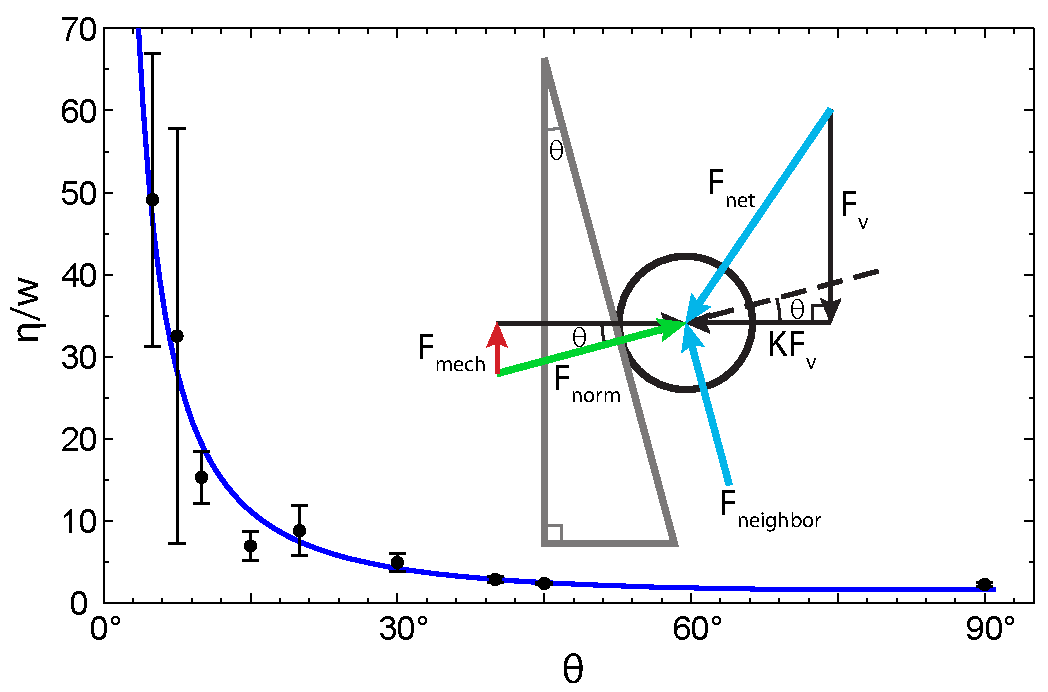
\includegraphics[width=\textwidth]{Figures/chapter2/etavtheta.pdf}
	\caption{Fitted values of characteristic filling height per container width is plotted against various angles of inclination. The data is fitted to our model of $\eta$ as a function of the angle of inclination $\theta$, as described in equation. Inset is an illustration of the interaction of forces necessary to create a mechanical friction that increases with increasing $\theta$. Consequently higher $\theta$ leads to lower $\eta$.}
	\label{fig:etavtheta}
\end{figure}

The emergence of Janssen-like behavior with sawtooth walls suggests that the geometry of the sidewalls allows them to support the load of the granular materials, even in the absence of friction with the particles.  If we continue to assume that we have a fixed $K$ relating the horizontal and vertical pressure then we can resolve the vertical force on the sawtooth sidewall as a geometric construction (Inset to Figure \ref{fig:etavtheta}). A particle pressed against a sawtooth experiences an average net force, $F_{net}$, from the particles around it and the conveyor belt. This can be decomposed into horizontal $F_{h}$ and vertical $F_{v}$ components related by $F_{h}=KF_{v}$.  To balance the forces on a particle pressed against the wall the sawtooth must exert a normal force of 
\begin{equation}
%
F_{norm} =  F_{net}\frac{K\cos\theta+\sin\theta}{\sqrt{K^{2}+1}}
\end{equation}
%
(green arrow in Figure \ref{fig:etavtheta} inset) and the particle below it must provide a force $F_{neighbor}$. We can in turn decompose $F_{norm}$ to find the vertical reaction force
%
\begin{equation}
F_{mech} = F_{net}\frac{(K/2)\sin2\theta +\sin^{2}\theta}{\sqrt{K^{2}+1}}
\end{equation}
%
(red vector). Since in the original formulation $\mu_{pw}$ serves to create a vertical reaction force in the walls we can redefine Equation \ref{eq:eta} as 
%
\begin{equation} 
\frac{\eta}{w}= \frac{F_{net}}{2 K F_{mech}} = \frac{\sqrt{K^{2} +1}}{K(K\sin2\theta +2\sin^2 \theta)}.
\label{eq:etaw}
\end{equation}
%
We plot $\eta/w$ as a function of $\theta$ in Figure \ref{fig:etavtheta}.  We find that Equation \ref{eq:etaw} well fits this data for all values of $\theta$ with a single fit parameter $K = 0.32 \pm0.02$. This value of $K$ indicates that the horizontal forces on the confining walls are $\simeq 1/3$ of the vertical forces that are directed to the bottom.  Experimental studies of 3D gravity compacted granular materials reported values in the range 0.2-0.8 dependent on measurement technique, material, and filling protocol \cite{janssen_versuche_1895, caughey_lateral_1951, sundaram_reassessment_1979, atewologun_experimental_1991, rusinek_experimental_2003}. As done in these studies, we have also employed the approximation that the stress ratio is constant. The fact that our data is well fit by a single parameter, $K$, which falls within this range suggests that our approximation is valid. 

%The fact that our data is well fit by a single $K$ which falls within this range suggests that the stress ratio is a material parameter unaffected by the wall geometry.

%We have demonstrated that in 2D friction-compacted granular systems the sliding friction demobilizes the particle-wall friction and so the granular system behaves as if it is frictionless. This is demonstrated in Figure \ref{fig:pressurevh} where the bottom pressure increases linearly with filling height for $\theta=0^{\circ}$. By changing the wall geometry to a sawtooth pattern we observe Janssen-like behavior; the bottom pressure saturates faster with increasing $\theta$, which is consistent with Equation \ref{eq:janssen}. Increasing the sawtooth angle is analogous to increasing the coefficient of particle-wall friction. We find that increasing the angle of inclination, $\theta$ decreases the scaled characteristic filling height, $\eta/w$, of the system. The functional dependence of $\eta/w$ as a function of $\theta$ is well described by our geometric model (Equation \ref{eq:etaw}).   
%
%\ericemph{Make a list of the conclusions in bullet form.  What should a reader take away from this paper.}
%1) high friction granular materials compacted by friction can be made to behave like a frictionless fluid
%
%2) by introducing sawtooth patterns in the side walls, we can recover the Janssen effect. 
%
%3) the angle of inclination of the sawtooth triangles determines the tangential forces that lead to the saturation of pressure 

%\ericemph{A second list of what this is useful for, maybe bring back buckling.  Buckling happens when the interparticle force is too high.  Control this with sawtooth walls.}

In this paper we have shown that vibrations due to dynamic friction in conveyor belt driven systems is sufficient to relax away tangential forces on straight side walls. Under such conditions, a granular system behaves like a hydrostatic system; the pressure at the bottom increases linearly with filling height.  However, a Janssen effect can be recovered if we use sawtooth walls to introduce mechanical friction.  We find that the dependence of saturation height on the angle of the sawtooth is well modeled by simple geometric arguments. 

These results have direct application to industrial processes involving the transport and containment of granular materials on cenveyor belts. Our results show that large stresses in high friction granular systems can be reduced by modifying the confining wall geometry. By reducing the interparticle stress one should observe a reduced probability of buckling in the system.  Further, a lower interparticle stress should reduce the energy required to break up a jammed system and lead to smoother flowing transport of material.  

While this study sheds light on the role of geometry in static, friction-compacted granular systems, the next chapter delves into its role in gravity-driven, obstructed granular flows in similarly quasi-two dimensional systems. More specifically, the study focuses on the nature of shock waves in granular flows around an obstruction whose geometry is varied systematically. Much like this study, Chapter III will take an experimental approach to study quasi 2D granular systems, but this time in flow.  